% Digital Logic Lab 9 ALU with Input Register
% Created: 2020-04-02, Megan Gordon

%==========================================================
%=========== Document Setup  ==============================

% Formatting defined by class file
\documentclass[11pt]{article}

% ---- Document formatting ----
\usepackage[margin=1in]{geometry}	% Narrower margins
\usepackage{booktabs}				% Nice formatting of tables
\usepackage{graphicx}				% Ability to include graphics

%\setlength\parindent{0pt}	% Do not indent first line of paragraphs 
\usepackage[parfill]{parskip}		% Line space b/w paragraphs
%	parfill option prevents last line of pgrph from being fully justified

% Parskip package adds too much space around titles, fix with this
\RequirePackage{titlesec}
\titlespacing\section{0pt}{8pt plus 4pt minus 2pt}{3pt plus 2pt minus 2pt}
\titlespacing\subsection{0pt}{4pt plus 4pt minus 2pt}{-2pt plus 2pt minus 2pt}
\titlespacing\subsubsection{0pt}{2pt plus 4pt minus 2pt}{-6pt plus 2pt minus 2pt}

% ---- Hyperlinks ----
\usepackage[colorlinks=true,urlcolor=blue]{hyperref}	% For URL's. Automatically links internal references.

% ---- Code listings ----
\usepackage{listings} 					% Nice code layout and inclusion
\usepackage[usenames,dvipsnames]{xcolor}	% Colors (needs to be defined before using colors)

% Define custom colors for listings
\definecolor{listinggray}{gray}{0.98}		% Listings background color
\definecolor{rulegray}{gray}{0.7}			% Listings rule/frame color

% Style for Verilog
\lstdefinestyle{Verilog}{
	language=Verilog,					% Verilog
	backgroundcolor=\color{listinggray},	% light gray background
	rulecolor=\color{blue}, 			% blue frame lines
	frame=tb,							% lines above & below
	linewidth=\columnwidth, 			% set line width
	basicstyle=\small\ttfamily,	% basic font style that is used for the code	
	breaklines=true, 					% allow breaking across columns/pages
	tabsize=3,							% set tab size
	commentstyle=\color{gray},	% comments in italic 
	stringstyle=\upshape,				% strings are printed in normal font
	showspaces=false,					% don't underscore spaces
}

% How to use: \Verilog[listing_options]{file}
\newcommand{\Verilog}[2][]{%
	\lstinputlisting[style=Verilog,#1]{#2}
}




%======================================================
%=========== Body  ====================================
\begin{document}

\title{ELC 2137 Lab 10: 7-Segment Display with Time-Division Multiplexing}
\author{Megan Gordon}

\maketitle


\section*{Summary}

This lab looks to expand on previous labs by expanding into larger systems with more modules. It allowed us to learn how to create an arithmetic logic unit (ALU) capable of a few operations using hexadecimal values. In completing this lab, the following skills were gained: ability to create and implement a D register with synchronous enable and asynchronous reset, ability to create and implement an arithmetic logic unit (ALU), ability to import and modify modules, and use them to design a modular system. 



\section*{Results}

Below are the simulations with ERTs for 2 modules (register and an ALU) and pictures of the board for each step in the operation list for on-board testing. 
\medskip

\begin{figure}[ht]\centering
	\begin{tabular}{l|rrrrrrrrrrr}
		Time (ns): & 0-5 & 5-10 & 10-15 & 15-20 & 20-25 & 25-30 & 30-35 & 35-40 & 40-45 & 45-50 & 50-55 \\
		\midrule 
		D (hex) & 0 & 0 & a & a & 3 & 3 & 0 & 0 & 0->6 & 6 & 6  \\
		clk & 0 & 1 & 0 & 1 & 0 & 1 & 0 & 1 & 0 & 1 & 0 \\
		en & 0 & 0 & 1 & 1 & 1->0 & 0->1 & 1->0 & 0 & 0->1 & 1 & 1 \\
		rst & 0 & 0->1 & 0 & 0 & 0 & 0 & 0 & 0 & 0 & 0 & 0 \\
		\midrule
		Q (hex) & X & X->0 & a & a & a & a & a & a & a & 6 & 6  \\
		\bottomrule
	\end{tabular}\medskip

	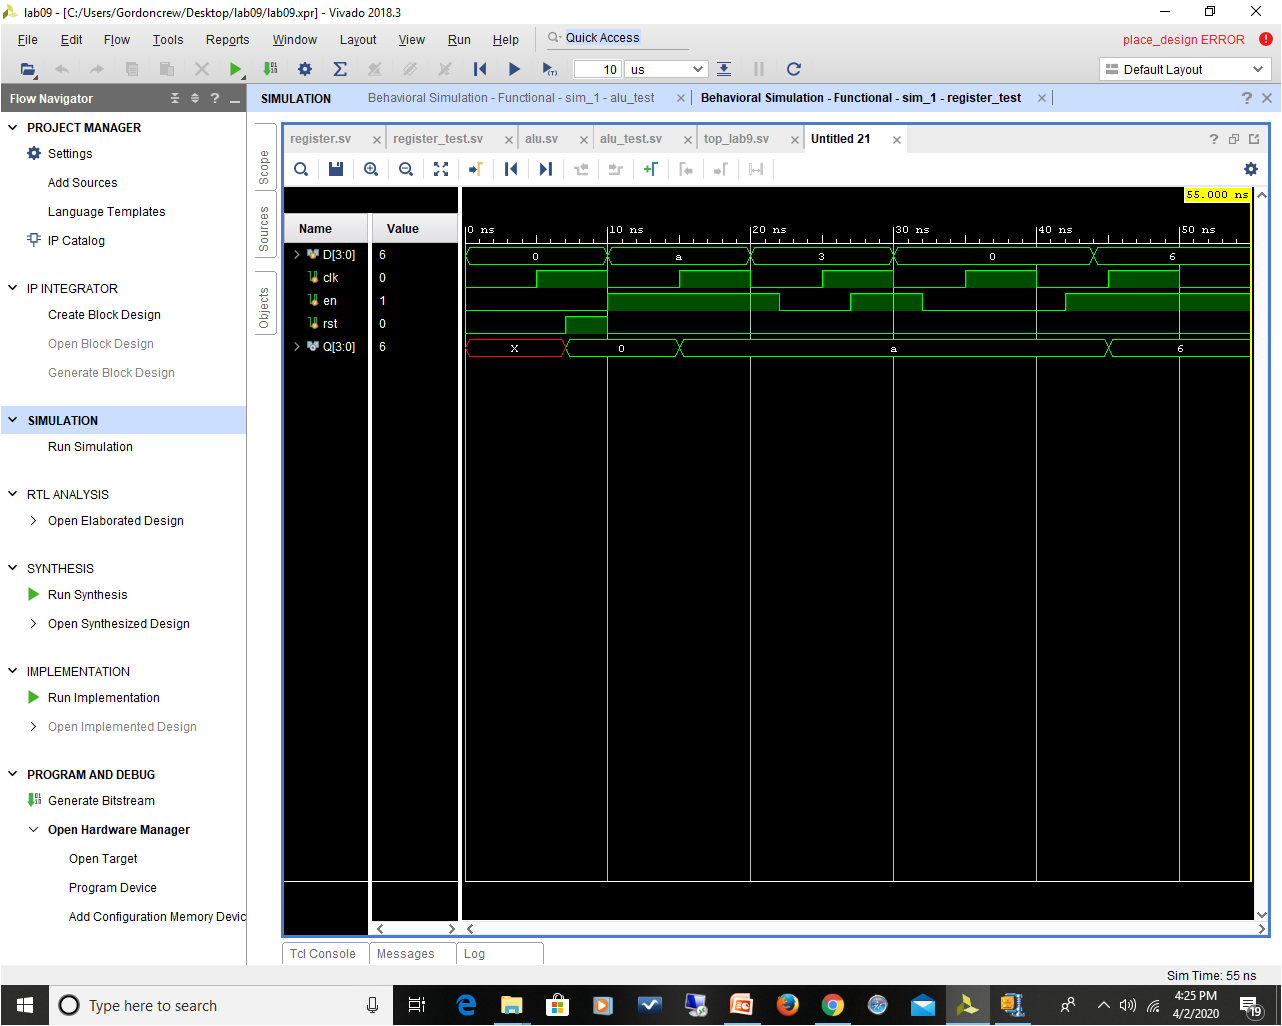
\includegraphics[width=1.15\textwidth, trim=5.6cm 12cm 0cm 3.5cm,clip]{register.png}
	\caption{Register ERT and Testbench Results}
	\label{fig:sim_with_table}
\end{figure}


\begin{figure}[ht]\centering
	\begin{tabular}{l|rrrrrr}
		Time (ns): & 0-10 & 10-20 & 20-30 & 30-40 & 40-50 & 50-60 \\
		\midrule
		in0 & 3 & 3 & 3 & 3 & 3 & 3 \\
		in1 & 2 & 2 & 2 & 2 & 2 & 2 \\
		op & 0 & 1 & 2 & 3 & 4 & 7 \\
		\midrule
		out & 5 & 1 & 6 & 3 & 1 & 3 \\
		\bottomrule
	\end{tabular}\medskip
	
	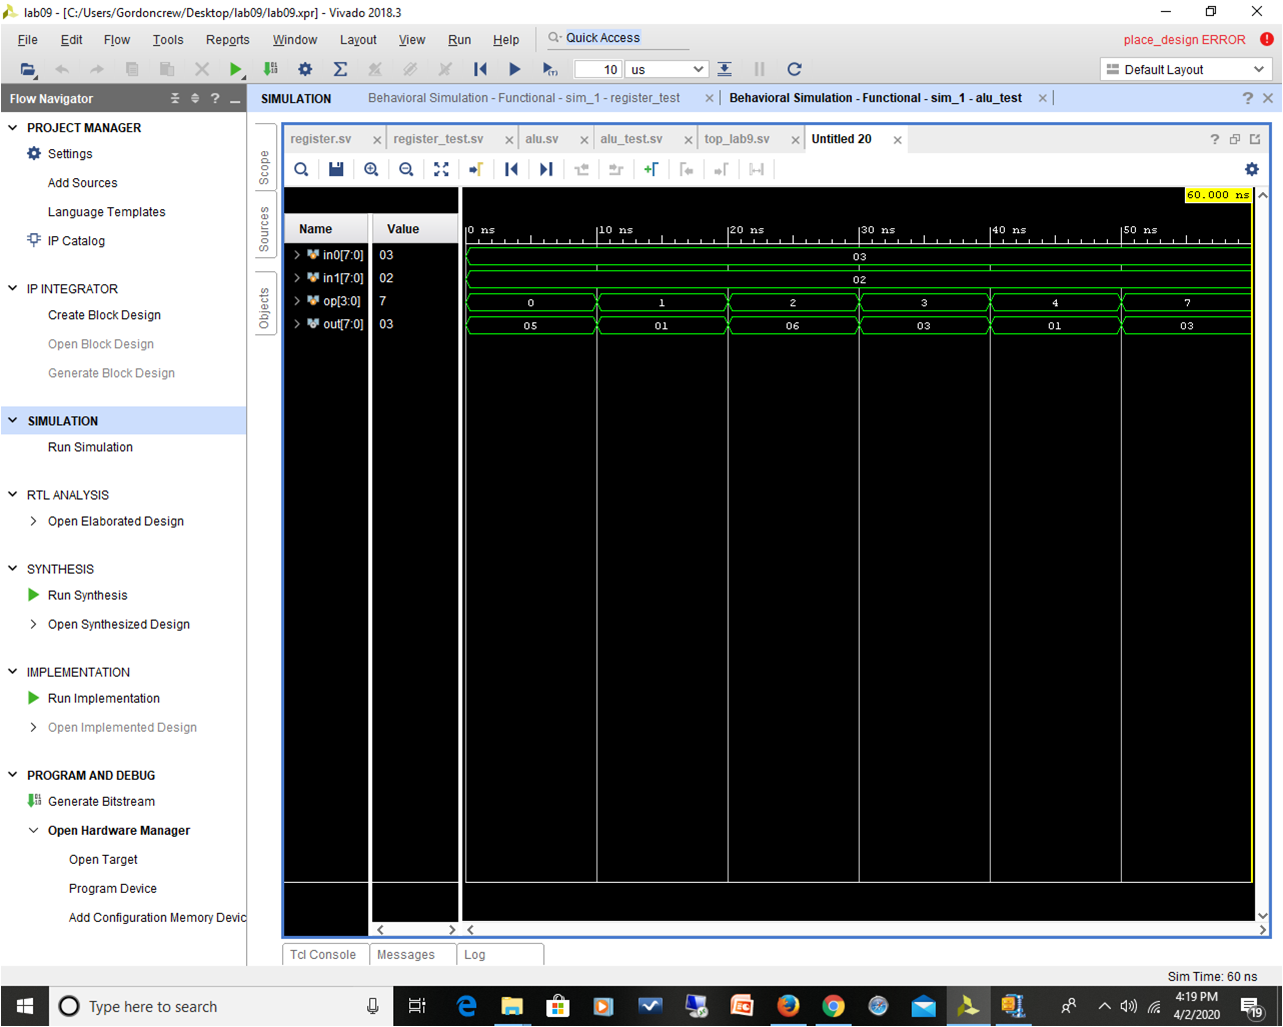
\includegraphics[width=1.15\textwidth, trim=5.8cm 12cm 0cm 4.0cm,clip]{alu.png}
	\caption{ALU ERT and Testbench Results}
	\label{fig:sim_with_table}
\end{figure}


\clearpage

\begin{figure}[ht]\centering
	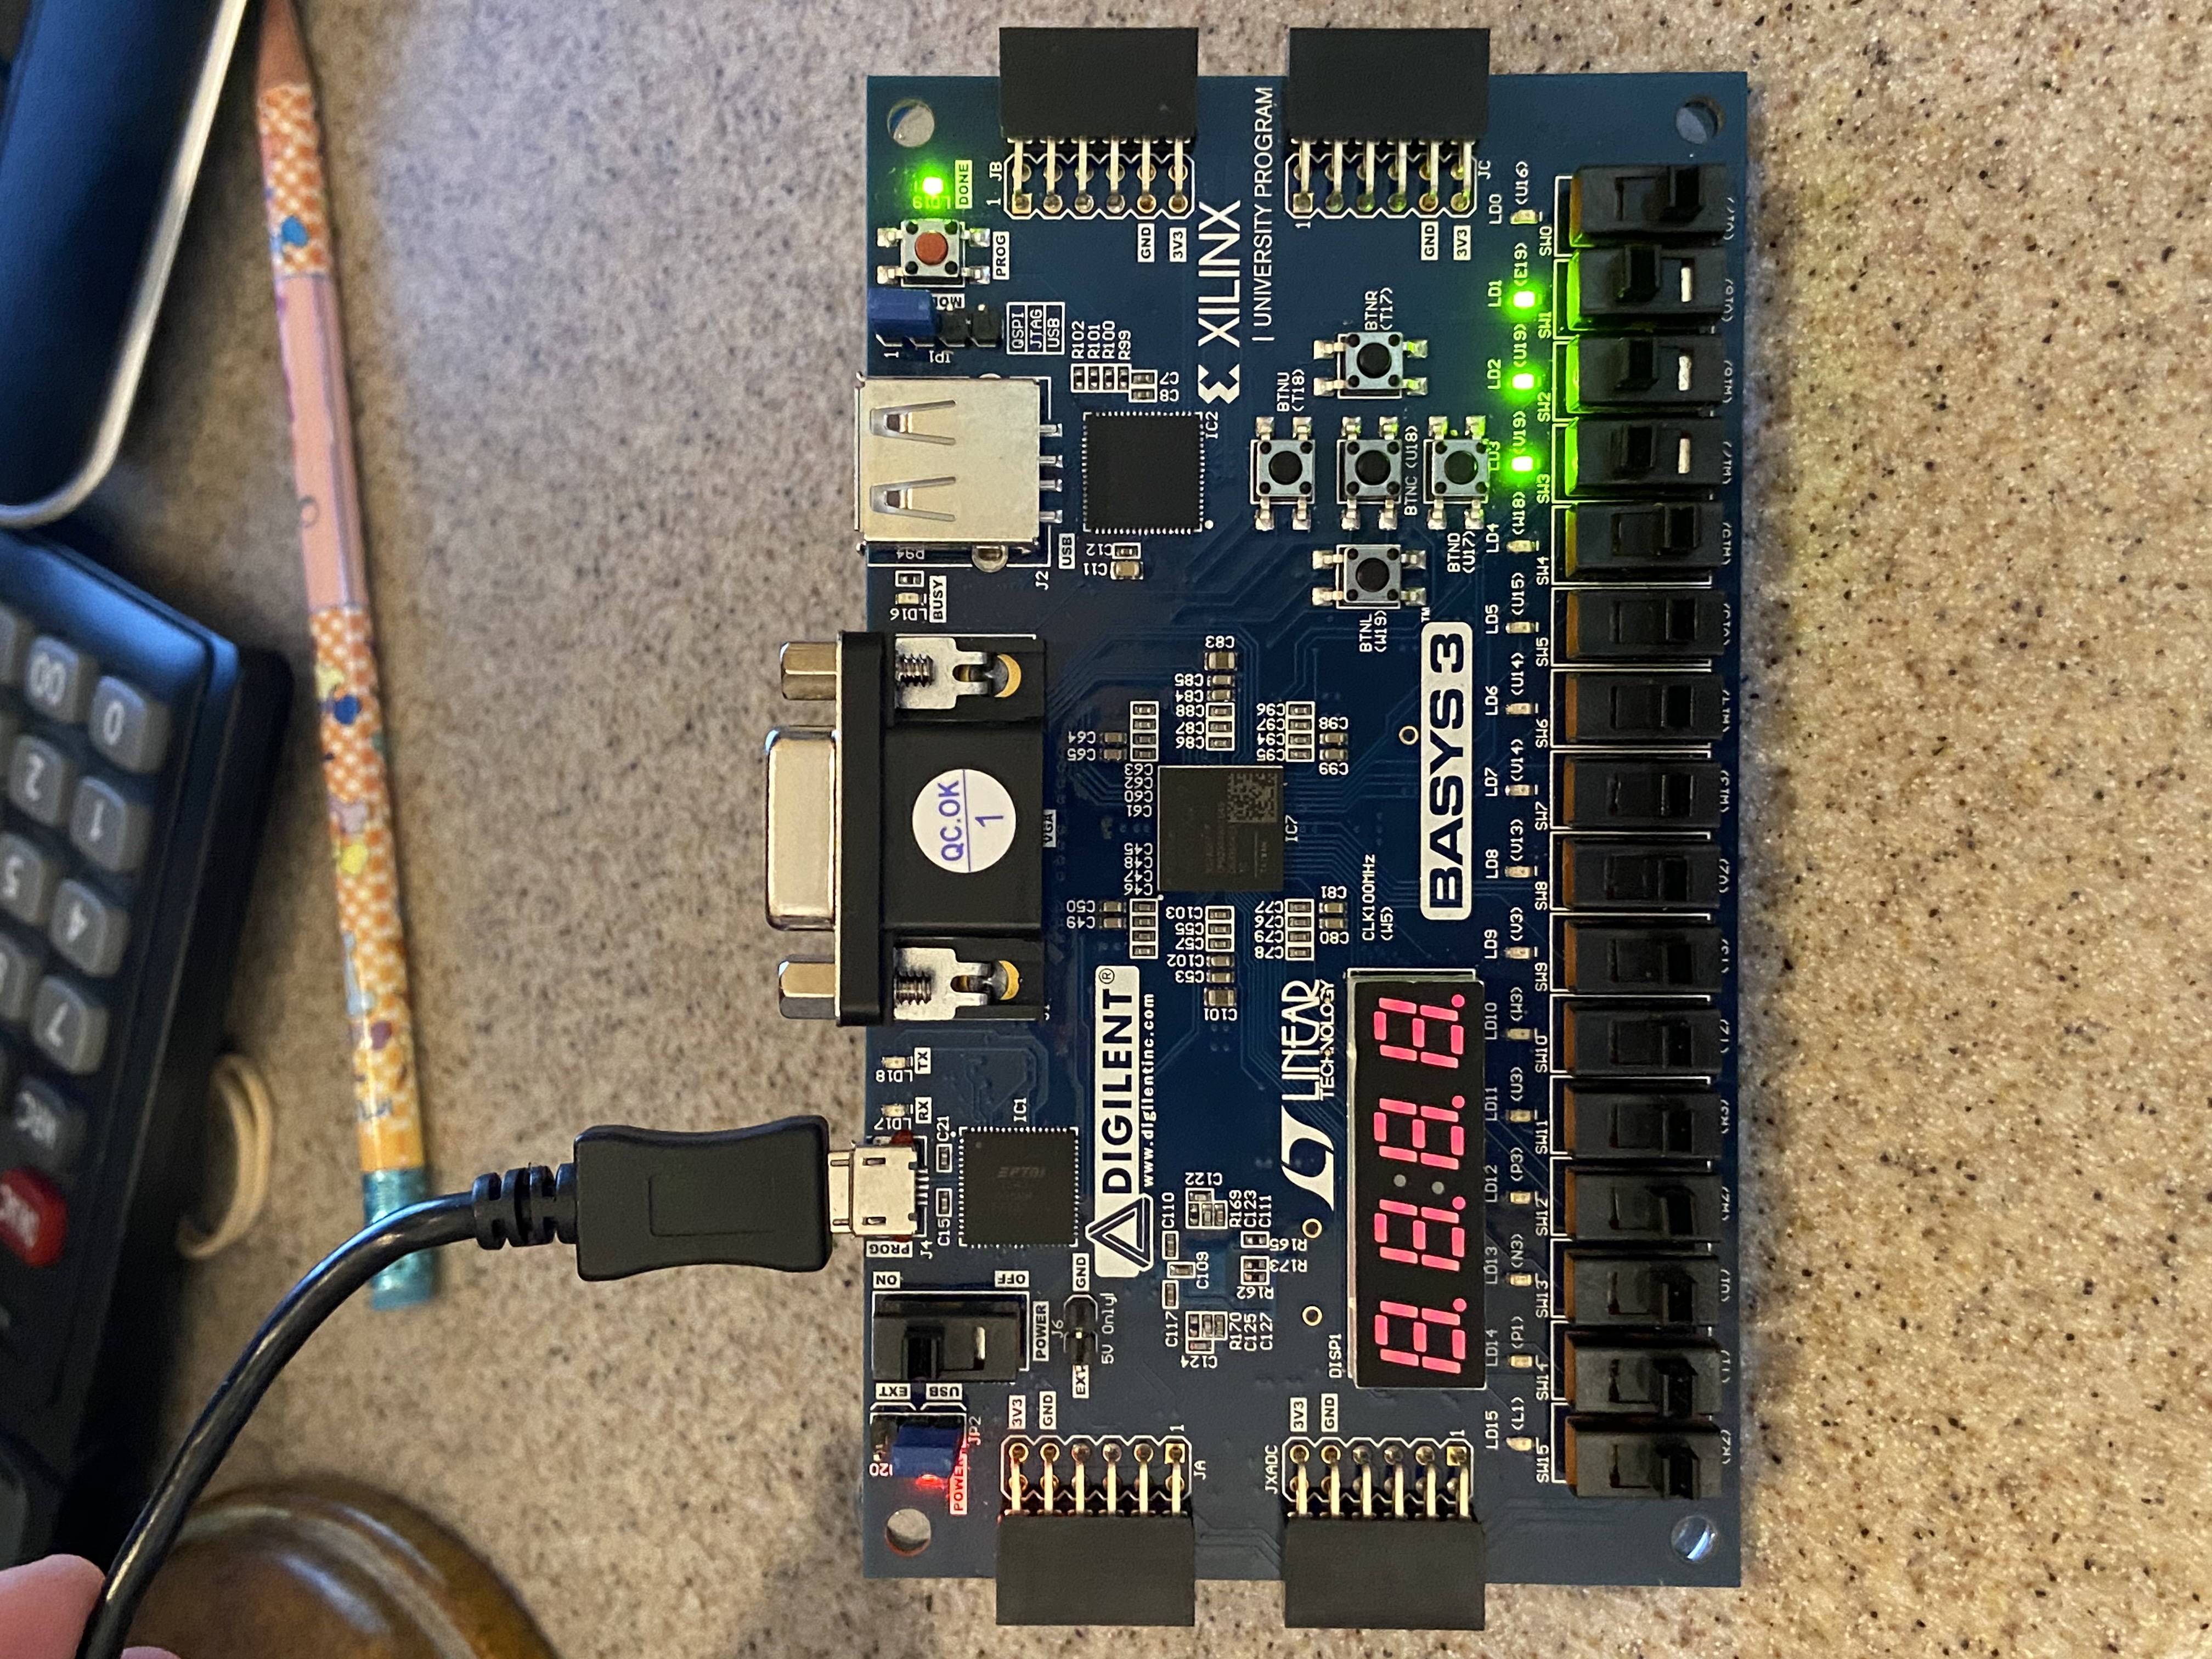
\includegraphics[angle=270, width=0.8\textwidth]{step1.jpg}
	\caption{Operation 1-Displaying hexadecimal "14"}
	\label{fig:sim_with_table}
\end{figure}
\clearpage

\begin{figure}[ht]\centering
	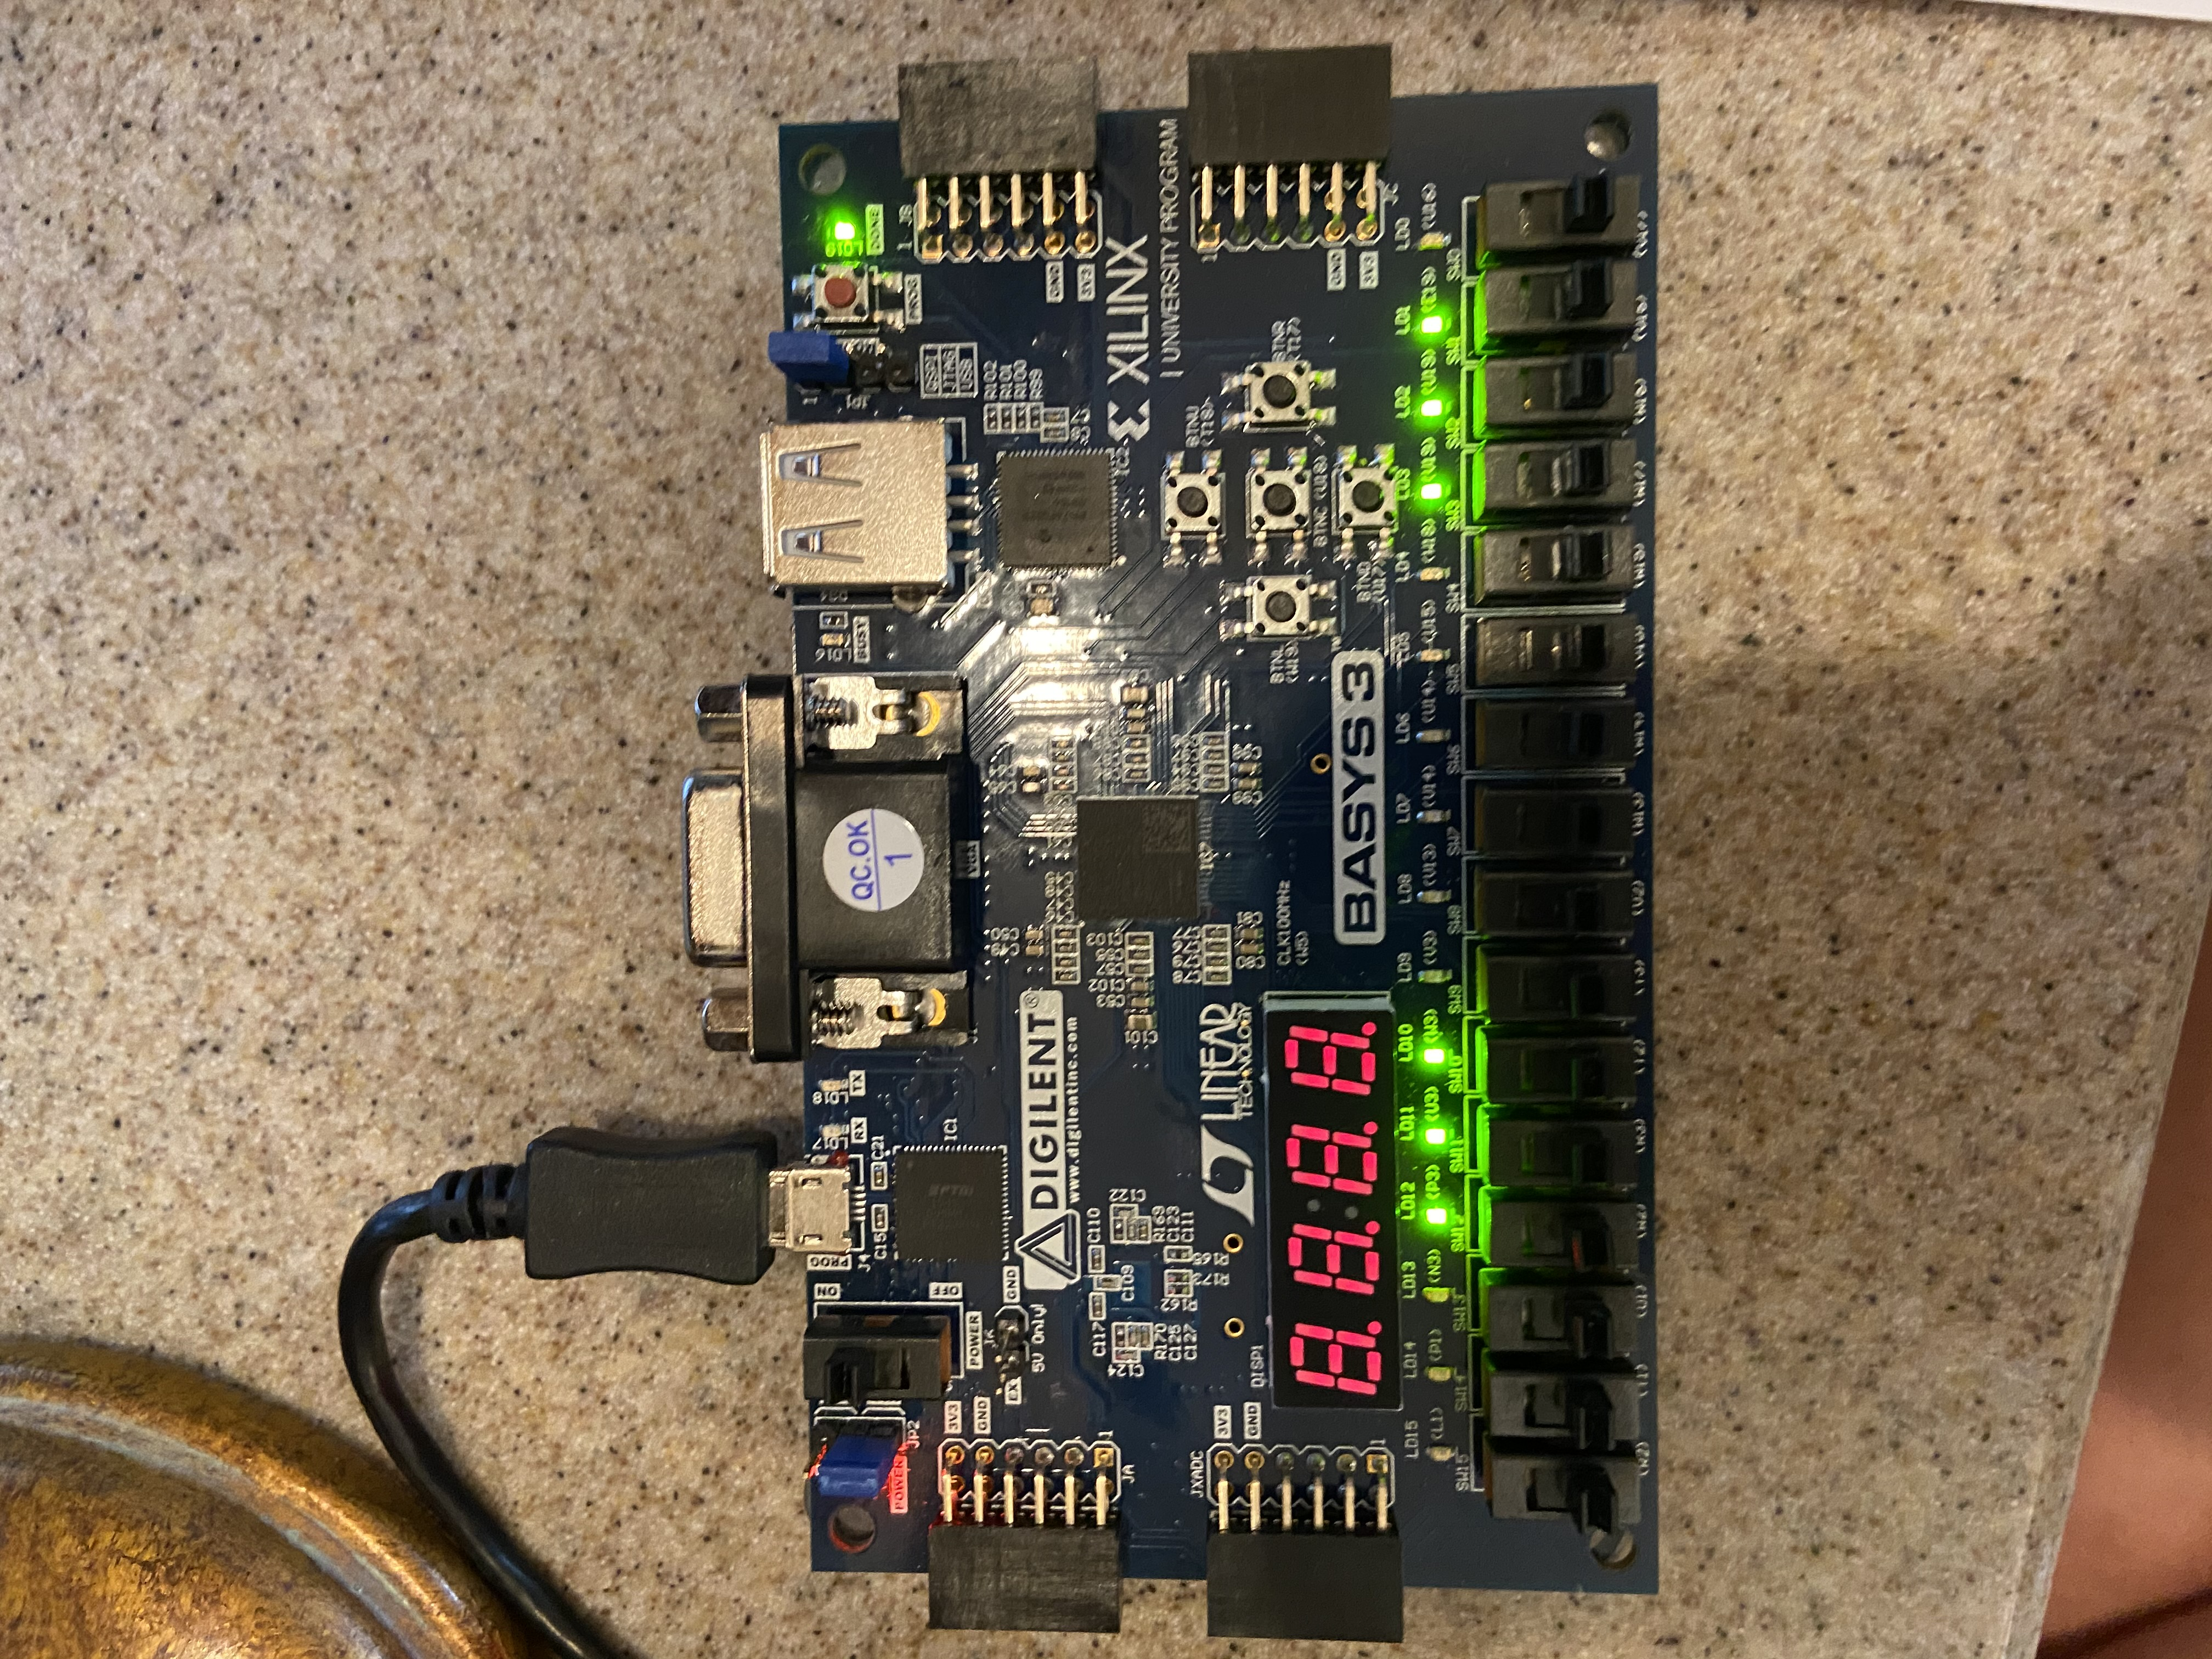
\includegraphics[angle=270, width=0.8\textwidth]{step2.jpg}
	\caption{Operation 2-Displaying hexdecimal "14" on LEDs 15-8 and 7-0}
	\label{fig:sim_with_table}
\end{figure}
\clearpage

\begin{figure}[ht]\centering
	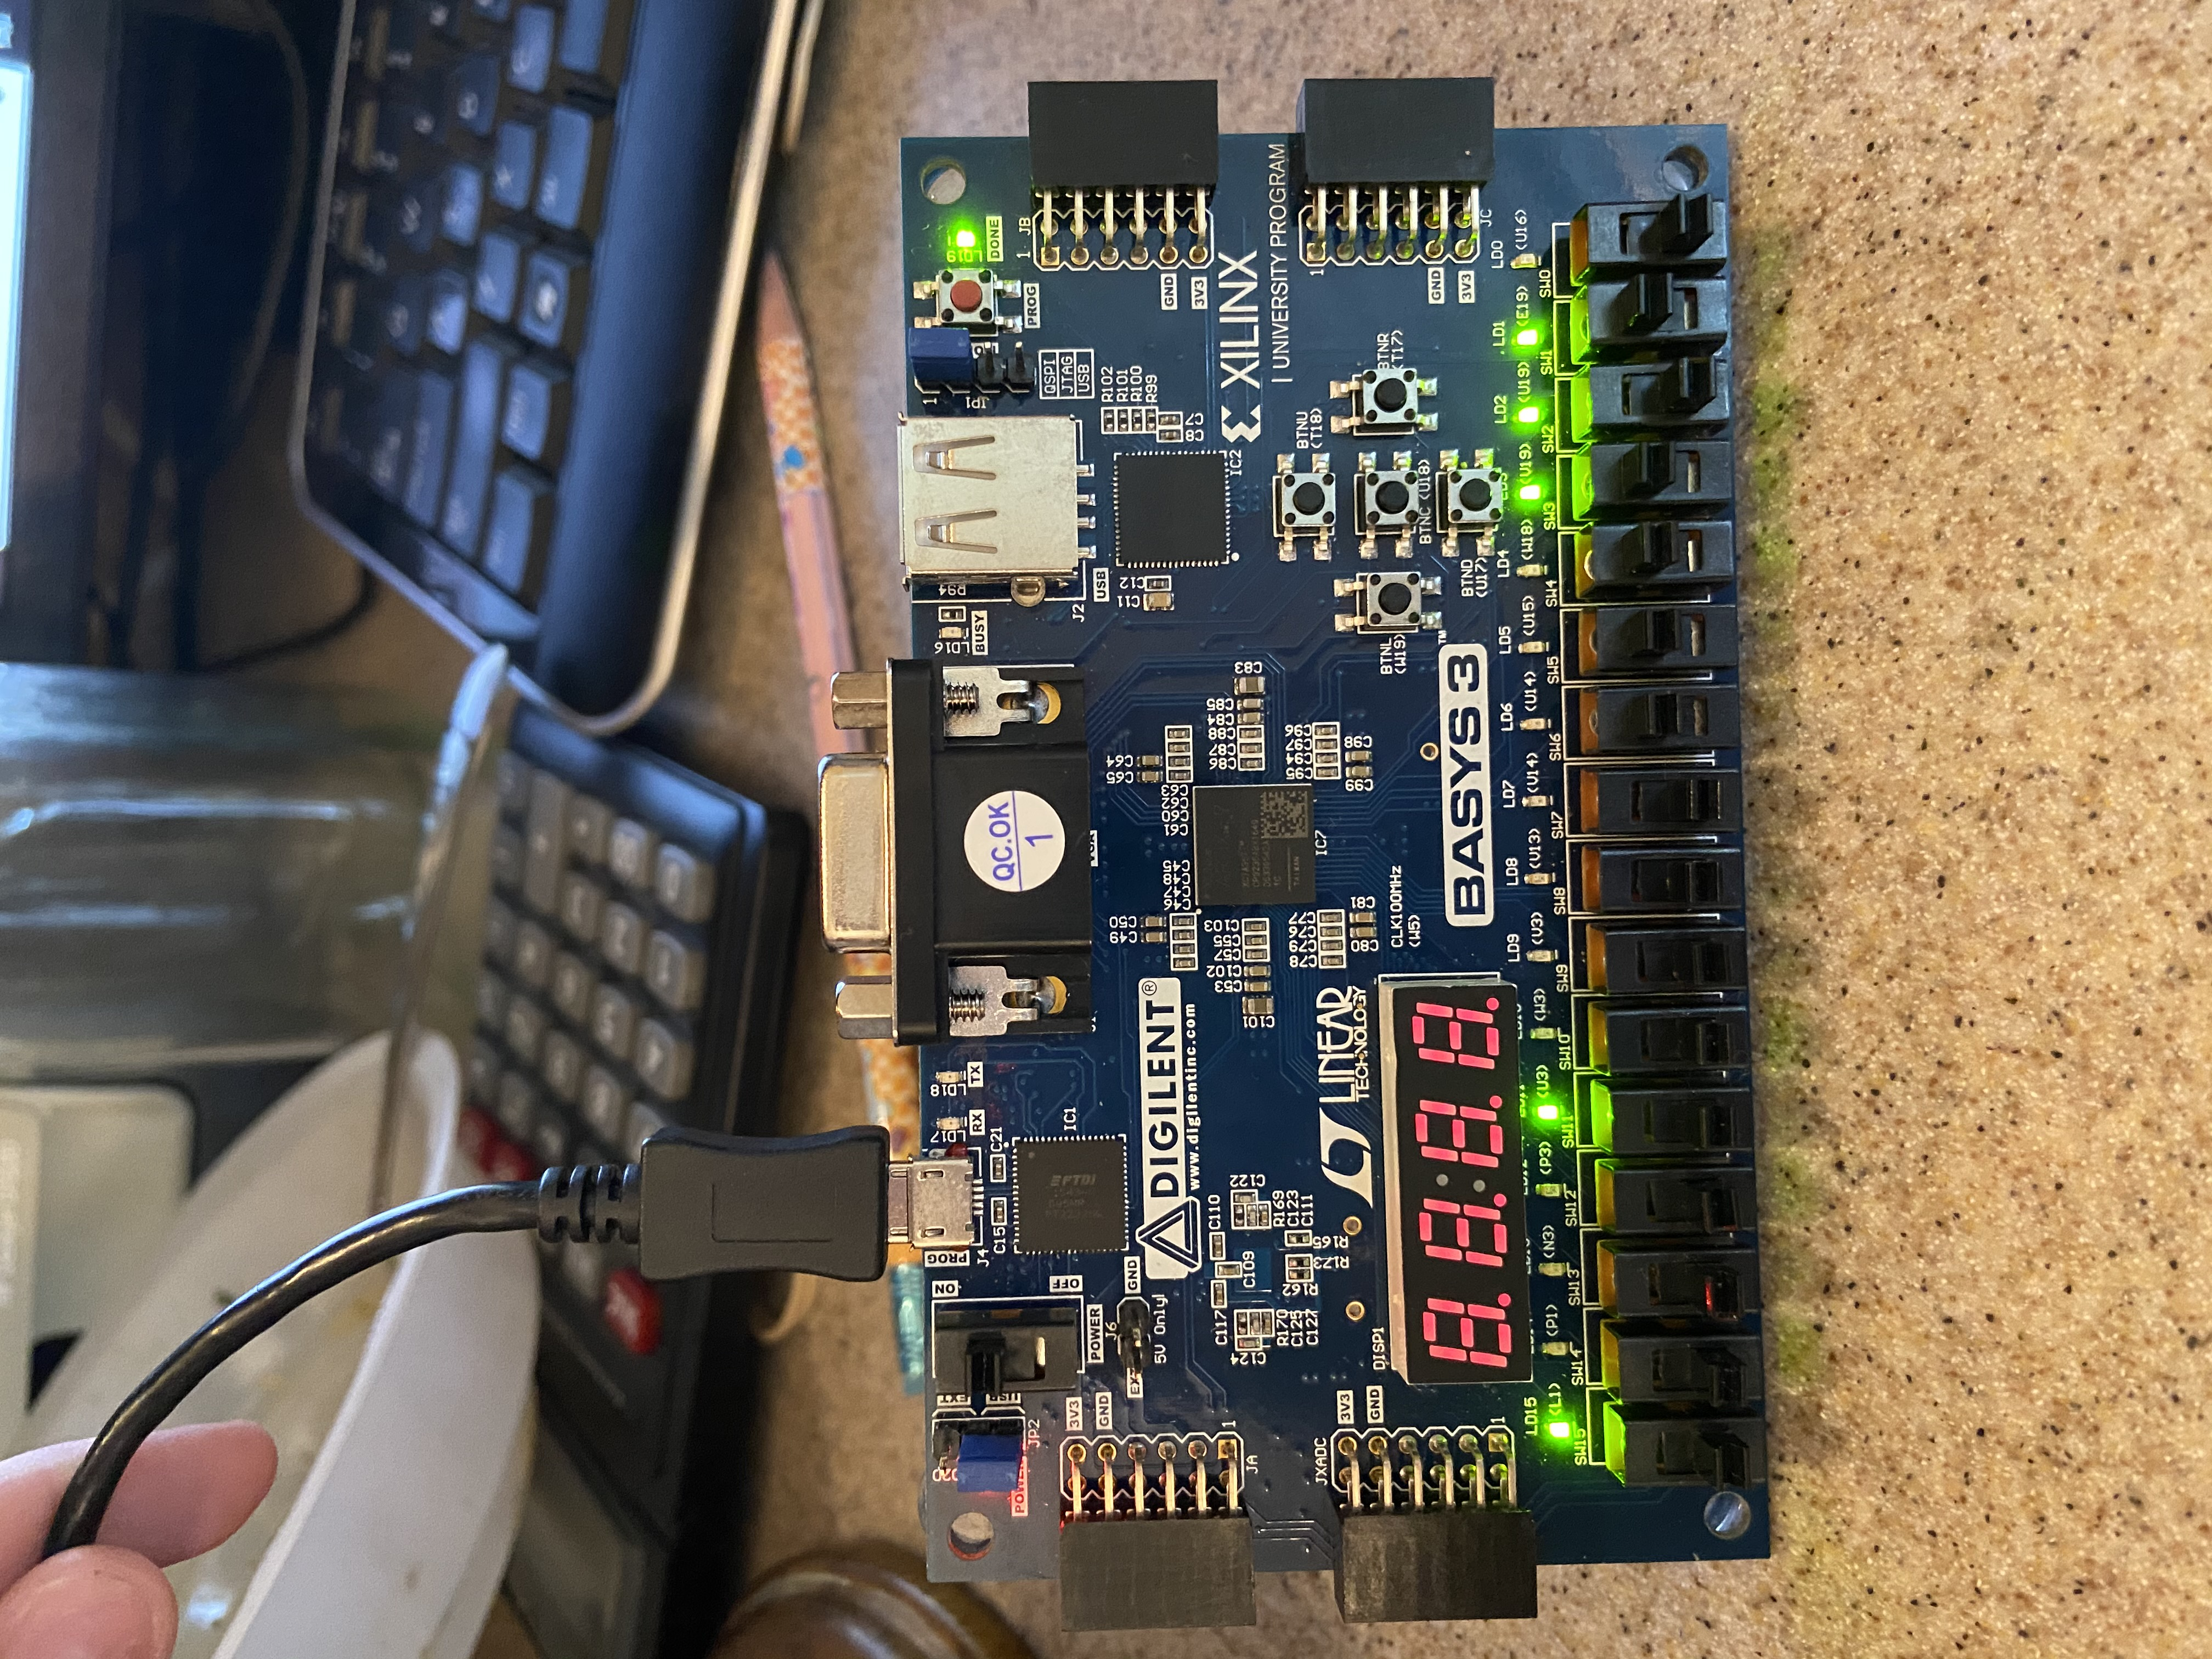
\includegraphics[angle=270, width=0.8\textwidth]{step3.jpg}
	\caption{Operation 3-Displaying sum of hexadecimal "14+7A"}
	\label{fig:sim_with_table}
\end{figure}
\clearpage





\section*{Code}

Code for source files for Register, ALU, and Top-Lab9 and for test bench files for Register and ALU is included below.

\begin{lstlisting}[style=Verilog,caption=Register Module Code,label=code:ex ]
`timescale 1ns / 1ps
//Megan Gordon, ELC 2137, 2020 -04 - 02

module register #(parameter N=1)(
				input clk, rst, en,
				input [N-1:0] D,
				output reg [N-1:0] Q
				);
				
				always @(posedge clk, posedge rst)
				begin
				if (rst==1)
				Q <= D;
				else if (en==1)
				Q <= D;
			end
endmodule
\end{lstlisting}

\begin{lstlisting}[style=Verilog,caption=ALU Module Code,label=code:ex ]
`timescale 1ns / 1ps
//Megan Gordon, ELC 2137, 2020 -04 - 02

module alu #(parameter N=8)
	(
	output reg[N-1:0] out,
	input [N-1:0] in0,
	input [N-1:0] in1,
	input [3:0] op
	);

	//parameters
	parameter ADD=0;
	parameter SUB=1;
	parameter AND=2;
	parameter OR=3;
	parameter XOR=4;

	always @*
	begin
		case(op)
			ADD: out = in0 + in1;
			SUB: out = in0 - in1;
			AND: out = in0 * in1;
			OR: out = in0 | in1;
			XOR: out = in0 ^ in1;
			default: out = in0;
		endcase
	end 

endmodule
\end{lstlisting}

\begin{lstlisting}[style=Verilog,caption=Top-Lab9 Module Code,label=code:ex ]
`timescale 1ns / 1ps
//Megan Gordon, ELC 2137, 2020 -04 - 02

module top_lab9(
input btnU,
input btnD,
input [11:0]sw,
input clk,
input btnC,
output [15:0]led
);

wire [7:0] Q1;
wire [7:0] out;
wire [7:0] Q2;   
wire [7:0] sw1;
wire [3:0] sw2;

assign sw1 = sw[7:0];
assign sw2 = sw[11:8];


register #(.N(8)) r1(.D(sw1), .clk(clk), 
		.en(btnD), .rst(btnC), .Q(Q1));

alu #(.N(8)) (.in0(sw1), .in1(Q1), 
		.op(sw2), .out(out));

register #(.N(8)) r2(.D(out), .clk(clk), 
		.en(btnU), .rst(btnC), .Q(Q2));

assign led [7:0] = Q1;
assign led [15:8] = Q2;       


endmodule
\end{lstlisting}

\begin{lstlisting}[style=Verilog,caption=Register Test Bench Code,label=code:ex ]
`timescale 1ns / 1ps
//Megan Gordon, ELC 2137, 2020 -04 - 02

module register_test();

reg [3:0] D;
reg clk, en, rst;
wire [3:0] Q;

register #(.N(4)) r(.D(D), .clk(clk), 
		.en(en), .rst(rst), .Q(Q));

	always begin 
		clk = ~clk; #5;
	end //clock constantly runs

	initial begin
		clk=0; en=0; rst=0; D=4'h0; #7;
		rst=1; #3; //reset
		D=4'hA; en=1; rst=0; #10
		D=4'h3; #2;
		en=0; #5;
		en=1; #3;
		D=4'h0; #2;
		en=0; #10;
		en=1; #2;
		D=4'h6; #11;
		$finish;
	end
              
endmodule
\end{lstlisting}

\begin{lstlisting}[style=Verilog,caption=ALU Test Bench Code,label=code:ex ]
`timescale 1ns / 1ps
//Megan Gordon, ELC 2137, 2020 -04 - 02

module alu_test();

reg [7:0] in0;
reg [7:0] in1;
reg [3:0] op;
wire [7:0] out;

alu #(.N(8)) r(.in0(in0), .in1(in1), 
		.op(op), .out(out));

	initial begin
		in0=3; in1=2; op=0; #10;
		in0=3; in1=2; op=1; #10;
		in0=3; in1=2; op=2; #10;
		in0=3; in1=2; op=3; #10;
		in0=3; in1=2; op=4; #10;
		in0=3; in1=2; op=7; #10;
		$finish;
	end

endmodule
\end{lstlisting}

\end{document}
